% BU ECE template for MS thesis and PhD dissertation.
%
%==========================================================================%
% MAIN PREAMBLE 
%==========================================================================%
\documentclass[12pt]{report}          % Single-sided printing for the library
%\documentclass[12pt,twoside]{report} % Double-sided printing
\usepackage[intlimits]{amsmath}
\usepackage{amsfonts,amssymb}
\DeclareSymbolFontAlphabet{\mathbb}{AMSb}
%\usepackage{natbib}
\usepackage{subfiles}
\usepackage{apalike}
\usepackage{float,subfigure}
\usepackage[bf]{caption}       
\setcaptionmargin{0.5in}
\usepackage{fancyheadings,fancybox,ifthen}
\usepackage{bu_ece_thesis}
\usepackage{url}
\usepackage{lscape,afterpage}
\usepackage{xspace}
\usepackage{color}
\usepackage{pdfpages}
%\usepackage{doi}
%==========================================================================%
%%% graphicx and pdf creation
\usepackage{graphicx}
\definecolor{gray}{RGB}{102,102,102}
\definecolor{mediumBlue}{RGB}{0,0,205}
%\usepackage{psfrag}
\DeclareGraphicsExtensions{.eps}   % extension for included graphics
%\usepackage{thumbpdf}              % thumbnails for ps2pdf
\usepackage[                       % hyper-references for ps2pdf
colorlinks=true,
linkcolor=mediumBlue,
citecolor=gray,
bookmarks=true,%                   % generate bookmarks ...
bookmarksnumbered=true,%           % ... with numbers
%hypertexnames=false,%              % needed for correct links to figures !!!
%breaklinks=true,%                  % breaks lines, but links are very small
%linkbordercolor={0,0,0},%          % blue frames around links
%pdfborder={0 0 112.0}				% border-width of frames 
]{hyperref}%  
%                                   % will be multiplied with 0.009 by ps2pdf
 \hypersetup{
  pdfauthor   = {Graham Voysey <gvoysey@bu.edu>},
  pdftitle    = {gvoysey-thesis.pdf},
  pdfsubject  = {Master's thesis},
  pdfkeywords = {biomedical engineering, hearing},
  pdfcreator  = {LaTeX/hyperref},
  pdfproducer = {LaTeX/P}
 }
%==========================================================================%
% customized commands can be placed here
%\newcommand{\figref}[1]{Figure~\ref{#1}}
%\newcommand{\chapref}[1]{Chapter~\ref{#1}}
%\newcommand{\latex}{\LaTeX\xspace}
%==========================================================================%

%==========================================================================%
% BEGIN
%==========================================================================%
\begin{document}

% The preliminary pages
% This file contains all the necessary setup and commands to create
% the preliminary pages according to the buthesis.sty option.

\title{Improved Brainstem Modeling to Characterize the Effect of Low Spontaneous Rate Fiber Loss on Auditory Neuropathy}

\author{Graham Voysey}

% Type of document prepared for this degree:
%   1 = Master of Science thesis,
%   2 = Doctor of Philisophy dissertation.
%   3 = Master of Science thesis and Doctor of Philisophy dissertation.
\degree=1

\prevdegrees{B.S., Boston University, 2006}

\department{Department of Biomedical Engineering}

% Degree year is the year the diploma is expected, and defense year is
% the year the dissertation is written up and defended. Often, these
% will be the same, except for January graduation, when your defense
% will be in the fall of year X, and your graduation will be in
% January of year X+1
\defenseyear{2016}
\degreeyear{2016}

% For each reader, specify appropriate label {First, second, third},
% then name, then title. Warning: If you have more than five readers
% you are out of luck, because it will overflow to a new page.
% Sometimes you may wish to put part of the title in with the name
\reader{First}{H. Steven Colburn, PhD}{Professor of Biomedical Engineering}
\reader{Second}{Barbara Shinn-Cunningham, PhD}{Professor of Biomedical Engineering}
\reader{Third}{Allyn E. Hubbard, PhD}{Professor of Electrical Engineering}

% The Major Professor is the same as the first reader, but must be
% specified again for the abstract page
\majorprof{H. Steven Colburn, PhD}{\mbox{Department of Biomedical Engineering}}

%                       PRELIMINARY PAGES
% According to the BU guide the preliminary pages consist of:
% title, copyright (optional), approval,  acknowledgments (opt.),
% abstract, preface (opt.), Table of contents, List of tables (if
% any), List of illustrations (if any). The \tableofcontents,
% \listoffigures, and \listoftables commands can be used in the
% appropriate places. For other things like preface, do it manually
% with something like \newpage\section*{Preface}.

% This is an additional page (do not hand it in at the library) to print
% boxed-in title, author and degree statement so that they are visible through
% the opening in BU covers used for reports. This makes a nicely bound copy.
%\buecethesistitleboxpage

% Make the titlepage based on the above information.  If you need
% something special and can't use the standard form, you can specify
% the exact text of the titlepage yourself.  Put it in a titlepage
% environment and leave blank lines where you want vertical space.
% The spaces will be adjusted to fill the entire page.
\maketitle
\cleardoublepage

% The copyright page is blank except for the notice at the bottom. You
% must provide your name in capitals.
\copyrightpage
\cleardoublepage

% Now include the approval page based on the readers information
\approvalpage
\cleardoublepage

% Here goes your favorite quote.
\newpage
\thispagestyle{empty}
% -*- root: ../gvoysey-thesis.tex -*-
\phantom{.}
\vspace{4in}

\begin{singlespace}
\begin{quote}
  We've heard a lot of models\ldots{}and heard suggested that we should take things out of our models to figure out what's important.  But in some sense, when I look at the diversity of models that have been presented so far---each of us leave out things.  So maybe in some sense we've got a start towards that approach.\\  
  
  So I can ask this question two ways, but let me ask it this way: \emph{What should we leave in?} What's the bare minimum we should leave in as we try to understand what's important about the function of the cochlea?
    % \textit{Facilis descensus Averni;}\\
  % \textit{Noctes atque dies patet atri janua Ditis;}\\*
  % \textit{Sed revocare gradum, superasque evadere ad auras,}\\
  % \textit{Hoc opus, hic labor est.}\hfill{Virgil (from Don's thesis!)}
  \vspace{2.5em}
  \begin{flushright}
  \textit{David C. Mountain\\Mechanics of Hearing (Attica, Greece 2014)}
  \end{flushright}
\end{quote}
\end{singlespace}
  

% \vspace{0.7in}
%
% \noindent
% [The descent to Avernus is easy; the gate of Pluto stands open night
% and day; but to retrace one's steps and return to the upper air, that
% is the toil, that the difficulty.]

\cleardoublepage

% The acknowledgment page should go here. Use something like
% \newpage\section*{Acknowledgments} followed by your text.
\newpage
\section*{\centerline{Acknowledgments}}
I would like to thank Jonathan Polimeni for cleaning up all these old
LaTeX style files and templates so that I didn't have to use Word to
write up this document. Also, I would like to thank all the CV/CNS lab
graduates for their contributions and tweaks to this organizational
scheme over the years (after many dissapointing interactions with
Martha Wellman).

This brings me to thank Martha Wellman of CAS and Brendon McDermot of
Mugar library who together uphold the stylistic and aesthetic
conventions that have been implemented in this LaTeX manuscript. Also
Sister Mary Virginia, the Thesis/dissertation coordinator of Mugar
Library, deserves some thanks as well.

Finally, I would like to thank Stephen Gildea, for the MIT sytle file
off which this current version is based, and Paolo Gaudiano for
porting the MIT style to one compatible for BU.

\cleardoublepage

% The abstractpage environment sets up everything on the page except
% the text itself.  The title and other header material are put at the
% top of the page, and the supervisors are listed at the bottom.  A
% new page is begun both before and after.  Of course, an abstract may
% be more than one page itself.  If you need more control over the
% format of the page, you can use the abstract environment, which puts
% the word "Abstract" at the beginning and single spaces its text.

\begin{abstractpage}
% ABSTRACT
My research is related to exploring the convergence of a recently discovered mechanism of hearing loss that is not detected in normal hearing tests called auditory neuropathy and the subjective phenomenon of tinnitus, or persistent ringing in the ears.   I have assembled a collection of models into a fuller simulation of this behavior, that helps to predict the likelihood and manner of maladaptive neuroplasticity in the brain that results from auditory neuropathy and may reflect a tinnitus state in humans. 
\end{abstractpage}
\cleardoublepage

% Now you can include a preface. Again, use something like
% \newpage\section*{Preface} followed by your text

% Table of contents comes after preface
\tableofcontents
\cleardoublepage

% If you have tables, uncomment the following line
%\listoftables
%\cleardoublepage

% If you have figures, uncomment the following line
\newpage
\listoffigures
\cleardoublepage

% List of Abbrevs is NOT optional (Martha Wellman likes all abbrevs listed)
\chapter*{List of Abbreviations}
\begin{center}
  \begin{tabular}{lll}
    \hspace*{2em} & \hspace*{1in} & \hspace*{4.5in} \\
    %CAD  & \dotfill & Computer-Aided Design \\   
    
  \end{tabular}
\end{center}
\cleardoublepage

% END OF THE PRELIMINARY PAGES

\newpage
\endofprelim
        
\cleardoublepage{}

% -*- root: ../gvoysey-thesis.tex -*-
\chapter{Introduction}
\label{chapter:Introduction}
\thispagestyle{myheadings}

\section{A brief history}
\label{sec:history}

Let's get started.

\cleardoublepage{}

% -*- root: ../gvoysey-thesis.tex -*-
\chapter{Literature Review}
\label{chapter:literaturereview}
\thispagestyle{myheadings}

% set this to the location of the figures for this chapter. it may
% also want to be ../Figures/2_Body/ or something. make sure that
% it has a trailing directory separator (i.e., '/')!
\graphicspath{{2_LiteratureReview/Figures/}}

\section{Cochlear Synaptopathy} % (fold)
\label{sec:cochlear_synaptopathy}

% section cochlear_synaptopathy (end)

\section{Physiology of the Auditory Nerve} % (fold)
\label{sec:physiology_of_the_auditory_nerve}
\subsection{Spontaneous Rates of Fibers} % (fold)
\label{sub:spontaneous_rates_of_fibers}

% subsection spontaneous_rates_of_fibers (end)
\subsection{Low Spontaneous Rate Fibers Suffer Selective Losses} % (fold)
\label{sub:low_spontaneous_rate_fibers_suffer_selective_losses}

% subsection low_spontaneous_rate_fibers_suffer_selective_losses (end)

\subsection{Current Controversies} % (fold)
\label{sub:current_controversies}
% subsection current_controversies (end)
% section physiology_of_the_auditory_nerve (end)

\section{Relevant Functional Neuroanatomy of the Auditory Midbrain} % (fold)
\label{sec:relevant_functional_neuroanatomy_of_the_auditory_midbrain}
\subsection{The Dorsal Cochlear Nucleus} % (fold)
\label{sub:the_dorsal_cochlear_nucleus}
\subsubsection{The Small Cap Area} % (fold)
\label{ssub:the_small_cap_area}

% subsubsection the_small_cap_area (end)
% subsection the_dorsal_cochlear_nucleus (end)
\subsection{The Ventral Cochlear Nucleus} % (fold)
\label{sub:the_ventral_cochlear_nucleus}

% subsection the_ventral_cochlear_nucleus (end)
\subsection{The Inferior Colliculus} % (fold)
\label{sub:the_inferior_colliculus}

% subsection the_inferior_colliculus (end)
% section functional_neuroanatomy_of_the_auditory_midbrain (end)

\section{Auditory Modeling Environments} % (fold)
\label{sec:auditory_modeling_environments}
\subsection{The Carney Models} % (fold)
\label{sub:the_carney_models}
\subsubsection{The Zilany and Bruce Models} % (fold)
\label{ssub:zilany_and_bruce_2009_2014}

% subsubsection zilany_and_bruce_2009_2014 (end)
\subsubsection{Modulation Transfer Functions in the Inferior Colliculus} % (fold)
\label{ssub:modulation_transfer_functions_in_the_inferior_colliculus}

% subsubsection modulation_transfer_functions_in_the_inferior_colliculus (end)
% subsection the_carney_models (end)

\subsection{The Verhulst Model} % (fold)
\label{sub:the_verhulst_model}

% subsection the_verhulst_model (end)

% section auditory_modeling_environments (end)

\section{Objective Measures of Cochlear Synaptopathy} % (fold)
\label{sec:objective_measures_of_cochlear_synaptopathy}

% section objective_measures_of_cochlear_synaptopathy (end)

\cleardoublepage{}

% -*- root: ../gvoysey-thesis.tex -*-
\chapter{Aims}
\label{chapter:Aims}
\thispagestyle{myheadings}

% set this to the location of the figures for this chapter. it may
% also want to be ../Figures/2_Body/ or something. make sure that
% it has a trailing directory separator (i.e., '/')!
\graphicspath{{3_Aims/Figures/}}

This thesis is dedicated to investigating the models of the peripheral and central auditory systems and the utility of their predictive abilities of cochlear synaptopathy. 

This project was divided into three aims.  First, developing a coherent modeling environment that combined two leading models of the auditory periphery into one software package where the efficacy of each model could be compared ``head to head.''  Second, to advance the state of the models of the auditory periphery by extending them with new capabilities supported by available anatomical and physiological research.  Third, to use the improved toolchain to explore the proposed mechanisms underlying psychophysical and large-scale electrophysiological studies of cochlear synaptopathy with higher fidelity.

\begin{enumerate}
	\item \textbf{Simulate the ABR response to a forward-masking task with variable SR contributions.}
	A modeling environment was created using Python.  It incorporates two peripheral models of the auditory system: the Zilany model \citep{Zilany2014Updated} and the Verhulst model \citep{}
	To accomplish this task, the Cochlea modeling environment \citep{Rudnicki2014Cochlea} was used to provide easy integration of the Zilany model. \citep{Zilany2014Updated}

	Further work to incorporate \cite{Verhulst2015Functional}, which perform better in broadband noise, will be performed so that the outputs of different AN models to the same stimuli may be directly compared.

	At the conclusion of this aim, direct comparisons between \cite{Zilany2014Updated} and \cite{Verhulst2015Functional} will have been performed.

	\item \textbf{Integrate improved brainstem models.}  

	We hypothesize that the current approach to IC modeling in \cite{Verhulst2015Functional} does not fully account for the responses to a low-SR knockout AN model, and consequently under-represents the effects on the ABR wave V that have been experimentally measured.  

	Several models that offer a better approach exist, among them a new model from \cite{Carney2015Speech} which provides multiple classes of IC neurons that were shown to track complex tones (vowel formants) in noise.  To guide the selection of model weights and connectivities, relevant neuro-anatomical literature will be consulted.  Crucially, studies by~\cite{Ryugo2008Projections} and others have shown selectivities in SR projections to the small cap of the DCN, which will guide modeling work by introducing specificities in weighting. Further, while the latency change trend is preserved between both the models proposed by \citeauthor{Zilany2014Updated} and \citeauthor{Verhulst2015Functional}, the magnitude of the effect is greatly different.  

	This discrepancy may be remedied by introduction of new IC modeling components, which are better incorporated in the \cite{Zilany2014Updated} model.
	
	\item \textbf{Relate model responses to psychophysical measures.}  

	We will compare subject Wave V latency data from \citeauthor{Mehraei2015Individual} and \citeauthor{Mehraei2016Auditory} as ground truth to the improved model output.
	
	
\end{enumerate}
\cleardoublepage{}

% -*- root: ../gvoysey-thesis.tex -*-
\chapter{Methods}
\label{chapter:Methods}
\thispagestyle{myheadings}

% set this to the location of the figures for this chapter. it may
% also want to be ../Figures/2_Body/ or something. make sure that
% it has a trailing directory separator (i.e., '/')!
\graphicspath{{4_Methods/Figures/}}

\section{Summary} % (fold)
\label{sec:summary}
This chapter gives a detailed description of the modeling environment created for this Thesis.  First, the configuration of the overall system is detailed.  Second, the configuration and use of two models of the auditory periphery are detailed.  Third, the creation of compound action potentials and population responses of the auditory nerve are given.  A method for the simulation of cochlear synaptopathy is also detailed, along with a new incorporation of a nonlinear distribution of auditory nerve fiber types as a function of center frequency.  Fourth, the use of these auditory nerve responses in simulation of the auditory brainstem and midbrain with two models are given, culminating in the creation of modeled Auditory Brainstem Responses.  Last, the utility of the system for large-scale simulation is shown. 
% section summary (end)

\section{Overview of Modeling Framework} % (fold)
\label{sec:overview_of_modeling_framework}
This section lays out the conceptual overview of the modeling framework created for this Thesis.  It is provisionally named ``Corti''\cite{Voysey2016Corti}, and is inspired by the EarLab project developed at Boston University as well as the ``Cochlea''\cite{Rudnicki2014Cochlea} modeling environment developed at the Technical University of Munich, from which it incorporates one peripheral model. 

\begin{figure}[htbp]
	\centering
	%\includegraphics[width=0.95\textwidth]{}
	\caption{Conceptual Overview of the Corti modeling environment.}
	\label{fig:corti-overview}
	\end{figure}

% section overview_of_modeling_framework (end)

\section{Peripheral Models} % (fold)
\label{sec:peripheral_models}
Two models of the auditory periphery are included: the transmission-line model by~\cite{Verhulst2015Functional} (henceforth ``The Verhulst model'') and the phenomenoligical model by~\cite{Zilany2014Updated} (henceforth ``The Zilany model'').

\subsection{The Verhulst Model} % (fold)
\label{sub:the_verhulst_model1}
The Verhulst model is useful for broadband stimuli.  It handles off-frequency effects (dispersion) well, and produces detailed information about many stages of sound propagation.  Otoacoustic emissions are also modeled. 
% subsection the_verhulst_model (end)
\subsection{The Zilany Model} % (fold)
\label{sub:the_zilany_model}
The implementation of the Zilany model here was adapted from~\cite{Rudnicki2014Cochlea}, who provided a python and C implementation that has been shown to produce identical output to the version documented by~\cite{Zilany2014Updated}. 

% subsection interoperability_of_the_zilany_and_verhulst_models (end)
\subsection{Interoperability of the Zilany and Verhulst Models} % (fold)
\label{sub:interoperability_of_the_zilany_and_verhulst_models}
The classification of SR types differs between the Zilany and Verhulst models in their firing rate classification cutoffs.  For the purposes of this work, both support combining the low- and medium- rate fibers into one population with mean spike rates less than 18 spikes/sec.  
% subsection the_zilany_model (end)

\subsection{Peripheral Model Output} % (fold)
\label{sub:peripheral_model_output}
The Verhulst model provides estimates of many behaviors of the auditory periphery.  The Zilany model provides some of the same. 

Both provide estimates of Instantaneous Firing Rate as a function of post-stimulus time for each combination of fiber type and best frequency, and these are passed to the next stage of the Corti environment.
% subsection peripheral_model_output (end)

% section peripheral_models (end)

\section{Auditory Nerve Response Models} % (fold)
\label{sec:auditory_nerve_response_models}
This stage of processing converts IFRs of specific fiber populations into an estimate of the summed activity of the auditory nerve. 

\subsection{Modeling Contributions of Inner Hair Cells} % (fold)
\label{sub:contributions_to_the_response_by_inner_hair_cells}
Along the Organ of Corti, each inner hair cell is innervated by multiple spiral ganglia.  The Verhulst and Zilany models, however, give responses of ``one'' fiber of each spontaneous rate type for each best center frequency, so modeling the summed response per IHC requires multiplicatively summing the responses of each SR type. 

Based on anatomical data, the Verhulst model assigns 19 fibers to each inner hair cell.  

The Zilany model's output is summed accordingly. 
% subsection contributions_to_the_response_by_inner_hair_cells (end)
\subsection{Weighting of IHC contribution} % (fold)
\label{sub:weighting_of_ihc_contribution}
The Verhulst model applies a scalar weighting factor to the summed Auditory Nerve Response using an undamaged nerve with 19 total fibers per IHC with 3 fibers for Low and Medium SR fibers and 13 High SR fibers. The scalar weighting factor was emmpirally chosen such that the modeled and summed response of IHCs with CFs logarithmically spaced between 175Hz and 20kHz produces a model ABR Wave-1 amplitude of 15 $\mu$V.  \citeauthor{Verhulst2015Functional} found the value of this weighting factor to be \num{0.15e-6} V $\times$ \num{2.7676e-07}.

To produce comparable results, the Zilany model was scaled accordingly. Using a small utility program which iteratively converged on a scaling factor with a tolerance of 1 nV, the scaling factor that produced an ABR Wave-1 amplitude of 15$\mu$V$\pm 1$nV was found to be \num{0.15e-6} V $\times$ \num{7.30282e-07}.
% subsection weighting_of_ihc_contribution (end)


\subsection{Weighting of Fiber Types per IHC} % (fold)
\label{sub:weighting_of_fiber_types_per_ihc}
Based on data from~\cite{Temchin2008Threshold}, the distribution of SR fiber types per IHC may not be uniform.  To account for this, fiber types may be weighted per IHC, rather than kept at the fixed 3-3-13 ratio set by Verhulst.  
\begin{figure}[htbp]
	\centering
	%\includegraphics[width=0.95\textwidth]{}
	\caption{Curve-fitting of experimental results by Temchin}
	\label{fig:temchin-curvefit}
\end{figure}

\subsubsection{Fractional weights}
A consequence of determining fiber percentages at each IHC from experimental data is that it's more appropriate to think of them as weighted contributions rather than integer number of spiral ganglia.  Non-integer values are normal.  This is OK in the context of summing everything into auditory nerve responses, but probably isn't for probing individual fibers.  The modeling environment does let individual fiber responses be saved at the earlier stage if that's a desired feature.
% subsection weighting_of_fiber_types_per_ihc (end)

\subsection{Modeling Synaptopathy} % (fold)
\label{sub:modeling_synaptopathy}
Selective degredation of the auditory nerve response is modeled by scaling each fiber type at each CF by a percentage factor.  

This will matter a lot when fiber types aren't linearlly allocated, and especially at high frequencies.
% subsection modeling_synaptopathy (end)
% section auditory_nerve_response_models (end)

\section{Brainstem Models} % (fold)
\label{sec:brainstem_models}
This section details the two brainstem models in use, given by~\cite{Nelson2004Phenomenological} and~\cite{Carney2015Speech}.

\subsection{The Nelson Carney 2004 Brainstem} % (fold)
\label{sub:the_nelson_carney_2004_brainstem}

% subsection the_nelson_carney_2004_brainstem (end)
\subsection{The Carney 2015 Brainstem} % (fold)
\label{sub:the_carney_2015_brainstem}

% subsection the_carney_2015_brainstem (end)
% section brainstem_models (end)

\section{Usage of the Modeling Environment} % (fold)
\label{sec:usage_of_the_modeling_environment}
\subsection{Automated Parameter Exploration} % (fold)
\label{sub:automated_parameter_exploration}

% subsection automated_parameter_exploration (end)
% section usage_of_the_modeling_environment (end)
\cleardoublepage{}

% -*- root: ../gvoysey-thesis.tex -*-
\chapter{Results}
\label{chapter:Results}
\thispagestyle{myheadings}

% set this to the location of the figures for this chapter. it may
% also want to be ../Figures/2_Body/ or something. make sure that
% it has a trailing directory separator (i.e., '/')!
\graphicspath{{5_Results/Figures/}}
\section{Chapter Summary} % (fold)
\label{sec:results_summary}
This chapter describes the results obtained when using the modeling environment described in~\autoref{chapter:Methods} to simulate a series of tone-in-noise experiments performed in humans by \citeauthor{Mehraei2016Auditory} to elucidate certain aspects of cochlear synaptopathy. 

% section results_summary (end)
\section{Tone in noise experiment} % (fold)
\label{sec:tone_in_noise}
The following parameters were 
\subsection{Stimuli} % (fold)
\label{sub:stimuli}
Following \citeauthor{Mehraei2015Auditory,Mehraei2016Auditory}, 6 stimului were programmatically generated and stored as WAV files with a sampling frequency of 100 kHz.  As shown in \autoref{fig:stimuli-used}, stimulus onset was delayed by 20 $\mu$s of silence, and then consisted of 80 dB SPL clicks with a repetition rate of 100 ms in the presence of gaussian noise at different signal to noise ratios. 

\begin{figure}[htbp]
	\centering
	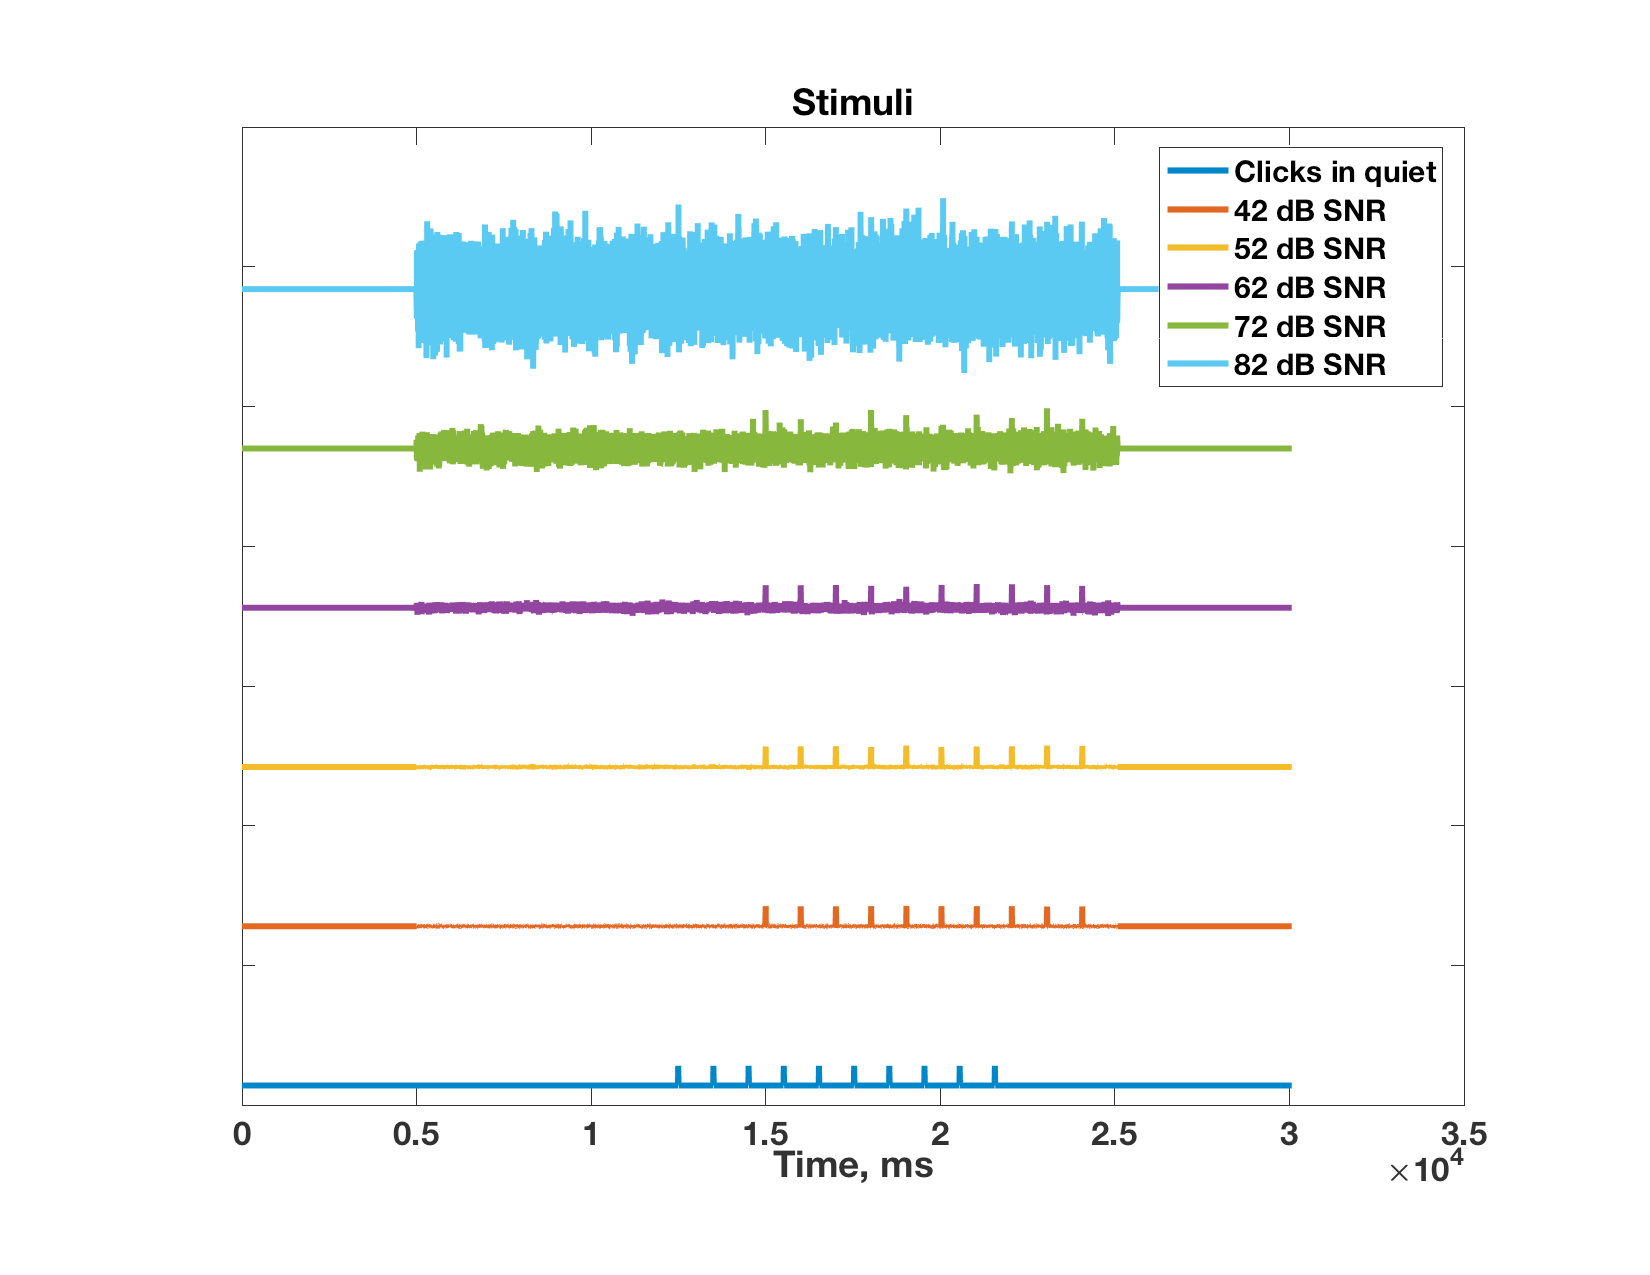
\includegraphics[width=0.95\textwidth]{stimuli-used.pdf}
	\caption[Experimental Stimuli]{Stimuli used to drive the auditory models.}
	\label{fig:stimuli-used}
\end{figure}
% subsection stimuli (end)

\begin{itemize}
	\item Ran the same stimului used by~\cite{Mehraei2015Auditory}: 80dB click, varying SNR
	\item Ran 1208 model configurations which varied  the stimulus SNR, the level and type of synaptopathy applied to the results, which peripheral model was used, whether the BM had any cf-weighting, and which brainstem model was used. 
	\item used a python library and cluster resources to make sure the results are easily searchable. 
	\item roughly 400 GB of model results.
	\item Can now examine the effects of individual parameter changes. 
	\item can now compare results to both prior modeling results and human data. 
\end{itemize}


\section{Simulations}
The experiment design tool described in \autoref{sec:automated_parameter_exploration} was used to specify a range of values for each parameter in Corti to reveal the relative contributions of each. 

In total, 240 separate simulations were run in parallel on Boston University's high-performance computing cluster over the course of approximately 9 days.  Model output was automatically stored into a HDF5 database approximately 250 GB in size.

\section{Effect of peripheral model} % (fold)
\label{sec:effect_of_peripheral_model}
The verhulst and zilany models will produce different estimates of the auditory nerve response. Prior work had their results very different; with recent changes to the verhulst model, this may have changed.
% section effect_of_peripheral_model (end)

\section{Effect of Synaptopathy} % (fold)
\label{sec:effect_of_synaptopathy}
Six kinds of synaptopathy were simulated: uniform and low-- and medium--SR specific losses of 10, 25, and 50 percent of each fiber type. 
% section effect_of_synaptopathy (end)

\section{Effect of CF weighting} % (fold)
\label{sec:effect_of_cf_weighting}
In models of the periphery that include more low SR fibers at high frequencies, synaptopathic losses will change.
% section effect_of_cf_weighting (end)

\section{Effect of brainstem model} % (fold)
\label{sec:effect_of_brainstem_model}
Does our intuition about a more physiologicaly relevant brainstem and midbrain model capturing more of the diversity of human responses bear out? 
% section effect_of_brainstem_model (end)
\cleardoublepage{}

% -*- root: ../gvoysey-thesis.tex -*-
\chapter{Discussion}
\label{chapter:Discussion}
\thispagestyle{myheadings}

% set this to the location of the figures for this chapter. it may
% also want to be ../Figures/2_Body/ or something. make sure that
% it has a trailing directory separator (i.e., '/')!
\graphicspath{{6_Discussion/Figures/}}
\section{Chapter Summary} % (fold)
\label{sec:discussion_summary}
This chapter compares the results obtained in this thesis with the human results obtained by \citeauthor{Mehraei2016Auditory}, and offers justifications and possible explanations for their similarities and differences.
% section discussion_summary (end)

\section{Comparison of Results to Prior Work} % (fold)
\label{sec:comparison_of_results_to_prior_work}
\subsection{Prior Models} % (fold)
\label{sub:prior_models}

% subsection prior_models (end)
\subsection{Prior Experimental Results} % (fold)
\label{sub:prior_experimental_results}

% subsection prior_experimental_results (end)
% section comparison_of_results_to_prior_work (end)

\section{Nonlinear behaviors in the Verhulst Model} % (fold)
\label{sec:nonlinear_behaviors_in_the_verhulst_model}
During the course of this work, an unexpected phenomenon was observed in the behavior of the Verhulst model in its response to stimuli of long duration.  In response to a sustained pure tone stimulus, the model predicts a strong response along the sections of the basilar membrane near the frequency of the pure tone.  Further, the model predicts small amplitude BM displacement at higher frequencies, reflecting dispersion of energies along the BM.  However, at the level of the IHC synapse, the off-frequency firing rate estimates are several times larger than the on-frequency response, and fall outside physiological boundaries.   

To relate basilar membrane displacement to IHC firing rates, the Verhulst model implements a three-store synaptic diffusion model adapted from~\cite{Westerman1988Diffusion} to have place-dependent initial values of vesicle state.   Following~\cite{Liberman1978AuditoryNerve}, the saturated firing rate of a hair cell was also adapted to be place-dependent and used as a reset threshold for the diffusion model parameters.  It is possible that in certain situations, this threshold is never reached and thus the firing rate estimate grows disproportionately.  

This behavior would potentially overestimate the off-frequency basal response to a sustained more apical stimulus.  However, some evidence exists \citep{Kiang1974Tails,Yates1990Basilar} that basal responses to apical stimuli can approach threshold in some cases. 
% section nonlinear_behaviors_in_the_verhulst_model (end)

\section{Consequences of percentage weighting degradation for synaptopathy} % (fold)
\label{sec:consequences_of_percentage_weighting_degradation_for_synaptopathy}
To obtain the total contribution of one inner hair cell, and thus one CF, to the population response of the AN, the model scales the responses of a low-, mid-, and high-spontaneous rate modeled fiber by three linear weights, thus reflecting what proportion of spiral ganglia belong to a given category for that IHC.  This approach makes two interrelated assumptions.  

First, it assumes that the spontaneous behavior of a given fiber is sufficiently similar to that of all others of its spontaneous rate category that it is not necessary to simulate each fiber individually.  In the case of the Verhulst model, this assumption is realistic.  However, the Zilany model may be configured to generate spontaneous activity pseudorandomly, so the firing statistics of a given fiber may differ both from others of its spontaneous rate class and from itself over sustained periods.  Second, as a result of the stochasticity of the Zilany model, it would potentially be informative to investigate the loss of individual fibers in a Monte Carlo simulation to address the variance in model responses.  This would further complicate simulation and increase the dimensionality of \emph{post-hoc} analysis. 

These assumptions make computation of AN responses practical: only three fibers per CF are modeled.  Using the default parameters that were used in this work, 3,000 fibers were simulated per model iteration.  Simulating each fiber individually would incur a tenfold increase in the number of fibers to simulate, suggesting that a full exploration of the parameter space, as was done in this work, would take approximately 90 days to compute.  
% section consequences_of_percentage_weighting_degradation_for_synaptopathy (end)

\section{Nonlinear Synaptopathic Models} % (fold)
\label{sec:nonlinear_synaptopathic_models}
The unexpectedly small effects of modeled synaptopathy on the overall model output may also be due to the uniformity of the synaptopathic impairment that was simulated.  While modeled impairment was specific to fibers of different spontaneous rates, it was applied uniformly over all CFs, as the variability of fiber type distribution per CF would impair some frequency ranges more than others for a given neuropathic condition. 

However, sensorineural hearing loss, particularly age-related hearing loss, is often specific to high frequencies while leaving low frequency bands largely unchanged.   Noise-induced or ototoxic hearing loss may have a narrower frequency band, leading to a notched audiogram while leaving other frequencies at normal thresholds, and models of synaptopathy that reflect these more complex losses may have more complex effects on simulation output.

The minimal changes in Wave I peak amplitude are expected.
citeauthor{Liberman2014Efferent} and others have demonstrated the robustness of audiometric thresholds in animals with as little as 20\% of the original hair cell population intact, so the preservation of the AN compound action potential is consistent even with very severe synaptopathies.
% section nonlinear_synaptopathic_models (end)
\cleardoublepage{}

% -*- root: ../gvoysey-thesis.tex -*-
\chapter{Conclusion}
\label{chapter:Conclusion}
\thispagestyle{myheadings}

% set this to the location of the figures for this chapter. it may
% also want to be ../Figures/2_Body/ or something. make sure that
% it has a trailing directory separator (i.e., '/')!
\graphicspath{{7_Conclusion/Figures/}}

\section{Chapter Summary} % (fold)
\label{sec:chapter_summary}

% section chapter_summary (end)


\cleardoublepage{}

%==========================================================================%
% Bibliography
\newpage
\singlespace{}
\bibliographystyle{jneurosci}

% each subdirectory can have its own BiBTeX file
\nocite{*}
\bibliography{Remote}
\cleardoublepage{}

%==========================================================================%
% Curriculum Vitae
% TODO -- uncomment this one day and check this symlink so that it points to the correct version of the CV. 
%\includepdf[pages={ - }]{0_Prelim/gvoysey-cv.pdf}

%==========================================================================%
\end{document}
 